\appendix

\section{1-loop prepotentials of 6d SCFTs on a circle with twist} \label{appendix:1-loop}

\subsection{Affine root system and 1-loop prepotential of W-bosons}\label{sec:App-affineroots}

In this appendix, we determine KK-momentum shifts for perturbative states in 6d theories. When a 6d gauge theory is compactified on a circle, the periodic boundary condition imposed on the gauge algebra $ \mathfrak{g} $ defines a map from $ S^1 $ to $ \mathfrak{g} $. The space of such map is generated by $ T_n^a =  T^a \otimes z^n $ for $ n \in \mathbb{Z} $ where $ T^a $ are the generators of $ \mathfrak{g} $ and $ z $ is the coordinate along $ S^1 $. The natural commutation relation is given by
\begin{align}
\comm*{T_n^a}{T_m^b} = \comm{T^a}{T^b} \otimes z^{n+m} = f^{abc} \,T_{n+m}^c\ ,
\end{align}
where $ f^{abc} $ is the structure constant of $ \mathfrak{g} $. This defines a loop algebra of $ \mathfrak{g} $, and its central extension is called an untwisted affine Lie algebra. Thus, a 6d gauge theory compactified on $ S^1 $ naturally has an affine Lie algebra structure. The untwisted affine Lie algebra for a simple Lie algebra of type $ X_\ell $ is denoted by $ X_\ell^{(1)}$. Dynkin diagrams of the untwisted affine Lie algebras $ X_\ell^{(1)}$ are drawn in Figure~\ref{fig:dynkin_untwist}, where the nodes of the Dynkin diagrams are labeled by the simple roots $\alpha_i$ ($i=1, \cdots, \ell$), while the affine node is labeled by $\alpha_0$. 

\begin{figure}[t]
	\centering
	\begin{subfigure}[b]{0.2\textwidth}
		\centering
		\begin{tikzpicture}
		\draw[thick] (0, 0) circle (0.1)
		(1.5, 0) circle (0.1);
		\draw[white, decoration={markings,mark=at position 1 with {\arrow[scale=3, black]{>}}},postaction={decorate}] (1,0) -- (1.2,0);
		\draw[white, decoration={markings,mark=at position 1 with {\arrow[scale=3, black]{>}}},postaction={decorate}] (1,0) -- (0.3,0);
		\draw[line width=1pt] (0.41, 0.07) -- (1.09, 0.07)
		(0.41, -0.07) -- (1.09, -0.07);
		\draw (0, -0.4) node {$ _1 $}
		(1.5, -0.4) node {$ _1 $};
		\draw (0, 0.4) node {$ \scriptstyle \alpha_0 $}
		(1.5, 0.4) node {$ \scriptstyle \alpha_1 $};
		\end{tikzpicture}
		\caption{$ A_1^{(1)} $}
		\vspace{3ex}
	\end{subfigure}
	\begin{subfigure}[b]{0.35\textwidth}
		\centering
		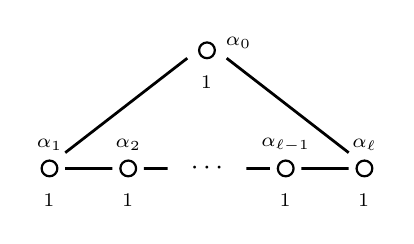
\begin{tikzpicture}
		\draw[thick] (0, 0) circle (0.1)
		(1, 0) circle (0.1)
		(2, 0) node {$ \cdots $}
		(3, 0) circle (0.1)
		(4, 0) circle(0.1)
		(2, 1.5) circle (0.1);
		\draw[line width=1pt] (0.2, 0) -- (0.8, 0)
		(1.2, 0) -- (1.5, 0)
		(2.5, 0) -- (2.8, 0)
		(3.2, 0) -- (3.8, 0)
		(0.2, 0.2) -- (1.75, 1.4)
		(3.8, 0.2) -- (2.25, 1.4);
		\draw (0, -0.4) node {$ _1 $}
		(1, -0.4) node {$ _1 $}
		(3, -0.4) node {$ _1 $}
		(4, -0.4) node {$ _1 $}
		(2, 1.1) node {$ _1 $};
		\draw (2.4, 1.6) node {$ \scriptstyle \alpha_0 $}
		(0, 0.3) node {$ \scriptstyle \alpha_1 $}
		(1, 0.3) node {$ \scriptstyle \alpha_2 $}
		(3, 0.3) node {$ \scriptstyle \alpha_{\ell-1} $}
		(4, 0.3) node {$ \scriptstyle \alpha_{\ell} $};
		\end{tikzpicture}
		\caption{$ A_{\ell}^{(1)} \ (\ell \geq 2) $}
		\vspace{3ex}
	\end{subfigure}
	\begin{subfigure}[b]{0.35\textwidth}
		\centering
		\begin{tikzpicture}
		\draw[thick] (0, 0) circle (0.1)
		(1, 0) circle (0.1)
		(2, 0) circle (0.1)
		(3, 0) node {$ \cdots $}
		(4, 0) circle (0.1)
		(5, 0) circle (0.1)
		(1, 1) circle (0.1);
		\draw[line width=1pt] (0.2, 0) -- (0.8, 0)
		(1.2, 0) -- (1.8, 0)
		(2.2, 0) -- (2.5, 0)
		(3.5, 0) -- (3.8, 0)
		(1, 0.2) -- (1, 0.8);
		\draw[white, decoration={markings,mark=at position 1 with {\arrow[scale=3, black]{>}}},postaction={decorate}] (4.5,0) -- (4.8,0);
		\draw[line width=1pt] (4.2, 0.07) -- (4.69, 0.07)
		(4.2, -0.07) -- (4.69, -0.07);
		\draw (0, -0.4) node {$ _1 $}
		(1, -0.4) node {$ _2 $}
		(2, -0.4) node {$ _2 $}
		(4, -0.4) node {$ _2 $}
		(5, -0.4) node {$ _1 $}
		(1.3, 1) node {$ _1 $}
		(5, -0.7) node {\textcolor{red}{$ _2 $}};
		\draw (0.6, 1) node {$ \scriptstyle \alpha_0 $}
		(0, 0.3) node {$ \scriptstyle \alpha_1 $}
		(0.7, 0.3) node {$ \scriptstyle \alpha_2 $}
		(2, 0.3) node {$ \scriptstyle \alpha_3 $}
		(4, 0.3) node {$ \scriptstyle \alpha_{\ell-1} $}
		(5, 0.3) node {$ \scriptstyle \alpha_{\ell} $};
		\end{tikzpicture}
		\caption{$ B_{\ell}^{(1)} \ (\ell \geq 3) $}
		\vspace{3ex}
	\end{subfigure}
	\hfill
	\begin{subfigure}[b]{0.4\textwidth}
		\centering
		\begin{tikzpicture}
		\draw[thick] (0, 0) circle (0.1)
		(1, 0) circle (0.1)
		(2, 0) node {$ \cdots $}
		(3, 0) circle (0.1)
		(4, 0) circle (0.1);
		\draw[line width=1pt] (1.2, 0) -- (1.5, 0)
		(2.5, 0) -- (2.8, 0);
		\draw[white, decoration={markings,mark=at position 1 with {\arrow[scale=3, black]{>}}},postaction={decorate}] (3.5, 0) -- (3.2, 0);
		\draw[white, decoration={markings,mark=at position 1 with {\arrow[scale=3, black]{>}}},postaction={decorate}] (0.5, 0) -- (0.8, 0);
		\draw[line width=1pt] (3.31, 0.07) -- (3.8, 0.07)
		(3.31, -0.07) -- (3.8, -0.07)
		(0.2, 0.07) -- (0.69, 0.07)
		(0.2, -0.07) -- (0.69, -0.07);
		\draw (0, -0.4) node {$ _1 $}
		(1, -0.4) node {$ _1 $}
		(3, -0.4) node {$ _1 $}
		(4, -0.4) node {$ _1 $}
		(1, -0.7) node {\textcolor{red}{$ _2 $}}
		(3, -0.7) node {\textcolor{red}{$ _2 $}};
		\draw (0, 0.3) node {$ \scriptstyle \alpha_{0} $}
		(1, 0.3) node {$ \scriptstyle \alpha_{1} $}
		(3, 0.3) node {$ \scriptstyle \alpha_{\ell-1} $}
		(4, 0.3) node {$ \scriptstyle \alpha_{\ell} $};
		\end{tikzpicture}
		\caption{$ C_{\ell}^{(1)} \ (\ell \geq 2) $}
		\vspace{3ex}
	\end{subfigure}
	\begin{subfigure}[b]{0.5\textwidth}
		\centering
		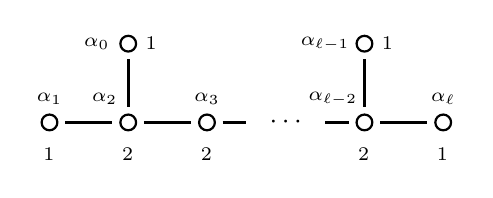
\begin{tikzpicture}
		\draw[thick] (0, 0) circle (0.1)
		(1, 0) circle (0.1)
		(2, 0) circle (0.1)
		(3, 0) node {$ \cdots $}
		(4, 0) circle (0.1)
		(5, 0) circle (0.1)
		(1, 1) circle (0.1)
		(4, 1) circle (0.1);
		\draw[line width=1pt] (0.2, 0) -- (0.8, 0)
		(1.2, 0) -- (1.8, 0)
		(2.2, 0) -- (2.5, 0)
		(3.5, 0) -- (3.8, 0)
		(4.2, 0) -- (4.8, 0)
		(1, 0.2) -- (1, 0.8)
		(4, 0.2) -- (4, 0.8);
		\draw (0, -0.4) node {$ _1 $}
		(1, -0.4) node {$ _2 $}
		(2, -0.4) node {$ _2 $}
		(4, -0.4) node {$ _2 $}
		(5, -0.4) node {$ _1 $}
		(1.3, 1) node {$ _1 $}
		(4.3, 1) node {$ _1 $};
		\draw (0.6, 1) node {$ \scriptstyle \alpha_{0} $}
		(0, 0.3) node {$ \scriptstyle \alpha_{1} $}
		(0.7, 0.3) node {$ \scriptstyle \alpha_{2} $}
		(2, 0.3) node {$ \scriptstyle \alpha_{3} $}
		(3.6, 0.3) node {$ \scriptstyle \alpha_{\ell-2} $}
		(3.5, 1) node {$ \scriptstyle \alpha_{\ell-1} $}
		(5, 0.3) node {$ \scriptstyle \alpha_{\ell} $};
		\end{tikzpicture}
		\caption{$ D_{\ell}^{(1)} \ (\ell \geq 4) $}
		\vspace{3ex}
	\end{subfigure}
	\hfill
	\begin{subfigure}[b]{0.4\textwidth}
		\centering
		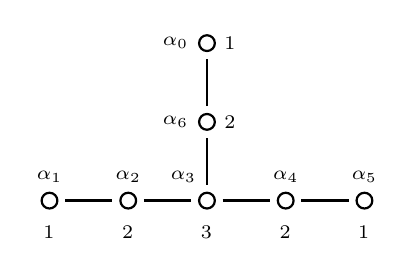
\begin{tikzpicture}
		\draw[thick] (0, 0) circle (0.1)
		(1, 0) circle (0.1)
		(2, 0) circle (0.1)
		(3, 0) circle (0.1)
		(4, 0) circle (0.1)
		(2, 1) circle (0.1)
		(2, 2) circle (0.1);
		\draw[line width=1pt] (0.2, 0) -- (0.8, 0)
		(1.2, 0) -- (1.8, 0)
		(2.2, 0) -- (2.8, 0)
		(3.2, 0) -- (3.8, 0)
		(2, 0.2) -- (2, 0.8)
		(2, 1.2) -- (2, 1.8);
		\draw (0, -0.4) node {$ _1 $}
		(1, -0.4) node {$ _2 $}
		(2, -0.4) node {$ _3 $}
		(3, -0.4) node {$ _2 $}
		(4, -0.4) node {$ _1 $}
		(2.3, 1) node {$ _2 $}
		(2.3, 2) node {$ _1 $};
		\draw (1.6, 2) node {$ \scriptstyle \alpha_{0} $}
		(0, 0.3) node {$ \scriptstyle \alpha_{1} $}
		(1, 0.3) node {$ \scriptstyle \alpha_{2} $}
		(1.7, 0.3) node {$ \scriptstyle \alpha_{3} $}
		(3, 0.3) node {$ \scriptstyle \alpha_{4} $}
		(4, 0.3) node {$ \scriptstyle \alpha_{5} $}
		(1.6, 1) node {$ \scriptstyle \alpha_{6} $};
		\end{tikzpicture}
		\caption{$ E_{6}^{(1)} $}
		\vspace{3ex}
	\end{subfigure}
	\begin{subfigure}[b]{0.5\textwidth}
		\centering
		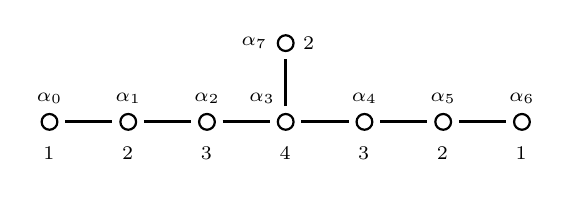
\begin{tikzpicture}
		\draw[thick] (0, 0) circle (0.1)
		(1, 0) circle (0.1)
		(2, 0) circle (0.1)
		(3, 0) circle (0.1)
		(4, 0) circle (0.1)
		(5, 0) circle (0.1)
		(6, 0) circle (0.1)
		(3, 1) circle (0.1);
		\draw[line width=1pt] (0.2, 0) -- (0.8, 0)
		(1.2, 0) -- (1.8, 0)
		(2.2, 0) -- (2.8, 0)
		(3.2, 0) -- (3.8, 0)
		(4.2, 0) -- (4.8, 0)
		(5.2, 0) -- (5.8, 0)
		(3, 0.2) -- (3, 0.8);
		\draw (0, -0.4) node {$ _1 $}
		(1, -0.4) node {$ _2 $}
		(2, -0.4) node {$ _3 $}
		(3, -0.4) node {$ _4 $}
		(4, -0.4) node {$ _3 $}
		(5, -0.4) node {$ _2 $}
		(6, -0.4) node {$ _1 $}
		(3.3, 1) node {$ _2 $};
		\draw (0, 0.3) node {$ \scriptstyle \alpha_{0} $}
		(1, 0.3) node {$ \scriptstyle \alpha_{1} $}
		(2, 0.3) node {$ \scriptstyle \alpha_{2} $}
		(2.7, 0.3) node {$ \scriptstyle \alpha_{3} $}
		(4, 0.3) node {$ \scriptstyle \alpha_{4} $}
		(5, 0.3) node {$ \scriptstyle \alpha_{5} $}
		(6, 0.3) node {$ \scriptstyle \alpha_{6} $}
		(2.6, 1) node {$ \scriptstyle \alpha_{7} $};
		\end{tikzpicture}
		\caption{$ E_{7}^{(1)} $}
		\vspace{3ex}
	\end{subfigure}
	\hfill
	\begin{subfigure}[b]{0.9\textwidth}
		\centering
		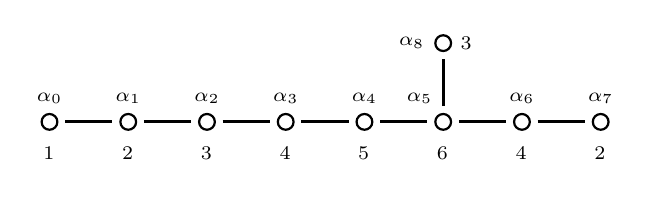
\begin{tikzpicture}
		\draw[thick] (0, 0) circle (0.1)
		(1, 0) circle (0.1)
		(2, 0) circle (0.1)
		(3, 0) circle (0.1)
		(4, 0) circle (0.1)
		(5, 0) circle (0.1)
		(6, 0) circle (0.1)
		(7, 0) circle (0.1)
		(5, 1) circle (0.1);
		\draw[line width=1pt] (0.2, 0) -- (0.8, 0)
		(1.2, 0) -- (1.8, 0)
		(2.2, 0) -- (2.8, 0)
		(3.2, 0) -- (3.8, 0)
		(4.2, 0) -- (4.8, 0)
		(5.2, 0) -- (5.8, 0)
		(6.2, 0) -- (6.8, 0)
		(5, 0.2) -- (5, 0.8);
		\draw (0, -0.4) node {$ _1 $}
		(1, -0.4) node {$ _2 $}
		(2, -0.4) node {$ _3 $}
		(3, -0.4) node {$ _4 $}
		(4, -0.4) node {$ _5 $}
		(5, -0.4) node {$ _6 $}
		(6, -0.4) node {$ _4 $}
		(7, -0.4) node {$ _2 $}
		(5.3, 1) node {$ _3 $};
		\draw (0, 0.3) node {$ \scriptstyle \alpha_{0} $}
		(1, 0.3) node {$ \scriptstyle \alpha_{1} $}
		(2, 0.3) node {$ \scriptstyle \alpha_{2} $}
		(3, 0.3) node {$ \scriptstyle \alpha_{3} $}
		(4, 0.3) node {$ \scriptstyle \alpha_{4} $}
		(4.7, 0.3) node {$ \scriptstyle \alpha_{5} $}
		(6, 0.3) node {$ \scriptstyle \alpha_{6} $}
		(7, 0.3) node {$ \scriptstyle \alpha_{7} $}
		(4.6, 1) node {$ \scriptstyle \alpha_{8} $};
		\end{tikzpicture}
		\caption{$ E_{8}^{(1)} $}
		\vspace{3ex}
	\end{subfigure}
	\hfill
	\begin{subfigure}[b]{0.5\textwidth}
		\centering
		\begin{tikzpicture}
		\draw[thick] (0, 0) circle (0.1)
		(1, 0) circle (0.1)
		(2, 0) circle (0.1)
		(3, 0) circle (0.1)
		(4, 0) circle (0.1);
		\draw[line width=1pt] (0.2, 0) -- (0.8, 0)
		(1.2, 0) -- (1.8, 0)
		(3.2, 0) -- (3.8, 0);
		\draw[white, decoration={markings,mark=at position 1 with {\arrow[scale=3, black]{>}}},postaction={decorate}] (2.5, 0) -- (2.8, 0);
		\draw[line width=1pt] (2.2, 0.07) -- (2.69, 0.07)
		(2.2, -0.07) -- (2.69, -0.07);
		\draw (0, -0.4) node {$ _1 $}
		(1, -0.4) node {$ _2 $}
		(2, -0.4) node {$ _3 $}
		(3, -0.4) node {$ _2 $}
		(4, -0.4) node {$ _1 $}
		(3, -0.7) node {\textcolor{red}{$ _4 $}}
		(4, -0.7) node {\textcolor{red}{$ _2 $}};
		\draw (0, 0.3) node {$ \scriptstyle \alpha_{0} $}
		(1, 0.3) node {$ \scriptstyle \alpha_{1} $}
		(2, 0.3) node {$ \scriptstyle \alpha_{2} $}
		(3, 0.3) node {$ \scriptstyle \alpha_{3} $}
		(4, 0.3) node {$ \scriptstyle \alpha_{4} $};
		\end{tikzpicture}
		\caption{$ F_4^{(1)} $}
	\end{subfigure}
	\begin{subfigure}[b]{0.4\textwidth}
		\centering
		\begin{tikzpicture}
		\draw[thick] (0, 0) circle (0.1)
		(1, 0) circle (0.1)
		(2, 0) circle (0.1);
		\draw[line width=1pt] (0.2, 0) -- (0.8, 0);
		\draw[white, decoration={markings,mark=at position 1 with {\arrow[scale=3, black]{>}}},postaction={decorate}] (1.5, 0) -- (1.8, 0);
		\draw[line width=1pt] (1.2, 0.07) -- (1.69, 0.07)
		(1.2, 0) -- (1.78, 0)
		(1.2, -0.07) -- (1.69, -0.07);
		\draw (0, -0.4) node {$ _1 $}
		(1, -0.4) node {$ _2 $}
		(2, -0.4) node {$ _1 $}
		(2, -0.7) node {\textcolor{red}{$ _3 $}};
		\draw (0, 0.3) node {$ \scriptstyle \alpha_{0} $}
		(1, 0.3) node {$ \scriptstyle \alpha_{2} $}
		(2, 0.3) node {$ \scriptstyle \alpha_{1} $};
		\end{tikzpicture}
		\caption{$ G_2^{(1)} $}
	\end{subfigure}
	\caption{Dynkin diagrams of untwisted affine Lie algebras $ X_\ell^{(1)} $. The number for each node is the dual Coxeter label (comark) $ d_i^\vee $. If a Coxeter label (mark) $ d_i $ differs from $ d_i^\vee $, it is represented as a red number. Dynkin diagrams without the affine node $ \alpha_0 $ reduce to the Dynkin diagrams of simple Lie algebras $ X_\ell $.} 
	\label{fig:dynkin_untwist}
\end{figure}

There is another type of affine Lie algebras. Lie algebras of types $ A_\ell $, $ D_\ell $ and $ E_6 $ have nontrivial outer automorphisms. Here, an outer automorphism on a Lie algebra $\mathfrak{g}$ is an automorphism which is not an inner automorphism, i.e., conjugation. An outer automorphism of Lie algebras can be viewed as a symmetry of their Dynkin diagrams. For Lie algebras of type $ A_\ell $, their Dynkin diagrams have a $ \mathbb{Z}_2 $ outer automorphism which exchanges the simple roots $ \alpha_i $ and $ \alpha_{\ell-i+1} $. For Lie algebras of type $ D_\ell $, Dynkin diagrams have a $ \mathbb{Z}_2 $ outer automorphism exchanging the simple roots $ \alpha_{\ell-1} $ and $ \alpha_{\ell} $. In particular, the Dynkin diagram of $ D_4 $ has a triality and thus $ D_4 $ algebra additionally has a $ \mathbb{Z}_3 $ outer automorphism whose action on the simple roots is given by $ \alpha_1 \to \alpha_2 \to \alpha_3 \to \alpha_1 $. For the Lie algebra of type $ E_6 $, its Dynkin diagram has a $ \mathbb{Z}_2 $ outer automorphism exchanging  $ \alpha_1 \leftrightarrow \alpha_5 $ and $ \alpha_2 \leftrightarrow \alpha_4 $.

Instead of imposing periodic boundary condition along $S^1$, one can impose twisted boundary condition using an outer automorphism of a simple Lie algebra $\mathfrak{g}$ associated with a gauge group of a 6d theory. That is to say, instead of considering a function $ f : \mathbb{R} \to \mathfrak{g} $ with $ f(x + 2\pi) = f(x) $, we introduce $ f(x + 2\pi) = \sigma(f(x)) $, where $ \sigma : \mathfrak{g} \to \mathfrak{g} $ is an automorphism. When $ \sigma $ is a non-trivial outer automorphism, the resultant loop algebra with central extension differs from untwisted affine Lie algebra. Such affine algebra is called a twisted affine Lie algebra, denoted by $ X_\ell^{(r)} $, where $ r = 2, 3 $ is the order of the automorphism in the Dynkin diagram. Dynkin diagrams of twisted affine Lie algebras are drawn in Figure~\ref{fig:dynkin_twist}.

\begin{figure}
\centering
\begin{subfigure}[b]{0.3\textwidth}
	\centering
	\begin{tikzpicture}
	\draw[thick] (0, 0) circle (0.1)
	(1.5, 0) circle (0.1);
	\draw[white, decoration={markings,mark=at position 1 with {\arrow[scale=3, black]{>}}},postaction={decorate}] (1,0) -- (0.3,0);
	\draw[line width=1pt] (0.42, 0.09) -- (1.09, 0.09)
	(0.37, 0.03) -- (1.09, 0.03)
	(0.37, -0.03) -- (1.09, -0.03)
	(0.42, -0.09) -- (1.09, -0.09);
	\draw (0, -0.4) node {$ _1 $}
	(1.5, -0.4) node {$ _2 $}
	(0, -0.7) node {\textcolor{red}{$ _2 $}}
	(1.5, -0.7) node {\textcolor{red}{$ _1 $}};
	\draw (0, 0.4) node {$ \scriptstyle \alpha_0 $}
	(1.5, 0.4) node {$ \scriptstyle \alpha_1 $};
	\end{tikzpicture}
	\caption{$ A_2^{(2)} $}
	\vspace{3ex}
\end{subfigure}
\begin{subfigure}[b]{0.6\textwidth}
	\centering
	\begin{tikzpicture}
	\draw[thick] (0, 0) circle (0.1)
	(1, 0) circle (0.1)
	(2, 0) node {$ \cdots $}
	(3, 0) circle (0.1)
	(4, 0) circle (0.1);
	\draw[line width=1pt] (1.2, 0) -- (1.5, 0)
	(2.5, 0) -- (2.8, 0);
	\draw[white, decoration={markings,mark=at position 1 with {\arrow[scale=3, black]{>}}},postaction={decorate}] (3.5, 0) -- (3.2, 0);
	\draw[white, decoration={markings,mark=at position 1 with {\arrow[scale=3, black]{>}}},postaction={decorate}] (0.5, 0) -- (0.2, 0);
	\draw[line width=1pt] (3.31, 0.07) -- (3.8, 0.07)
	(3.31, -0.07) -- (3.8, -0.07)
	(0.31, 0.07) -- (0.8, 0.07)
	(0.31, -0.07) -- (0.8, -0.07);
	\draw (0, -0.4) node {$ _1 $}
	(1, -0.4) node {$ _2 $}
	(3, -0.4) node {$ _2 $}
	(4, -0.4) node {$ _2 $}
	(0, -0.7) node {\textcolor{red}{$ _2 $}}
	(4, -0.7) node {\textcolor{red}{$ _1 $}};
	\draw (0, 0.3) node {$ \scriptstyle \alpha_{0} $}
	(1, 0.3) node {$ \scriptstyle \alpha_{1} $}
	(3, 0.3) node {$ \scriptstyle \alpha_{\ell-1} $}
	(4, 0.3) node {$ \scriptstyle \alpha_{\ell} $};
	\end{tikzpicture}
	\caption{$ A_{2\ell}^{(2)} \ ( \ell \geq 2) $}
	\vspace{3ex}
\end{subfigure}
\hfill
\begin{subfigure}[b]{0.45\textwidth}
	\centering
	\begin{tikzpicture}
	\draw[thick] (0, 0) circle (0.1)
	(1, 0) circle (0.1)
	(2, 0) circle (0.1)
	(3, 0) node {$ \cdots $}
	(4, 0) circle (0.1)
	(5, 0) circle (0.1)
	(1, 1) circle (0.1);
	\draw[line width=1pt] (0.2, 0) -- (0.8, 0)
	(1.2, 0) -- (1.8, 0)
	(2.2, 0) -- (2.5, 0)
	(3.5, 0) -- (3.8, 0)
	(1, 0.2) -- (1, 0.8);
	\draw[white, decoration={markings,mark=at position 1 with {\arrow[scale=3, black]{>}}},postaction={decorate}] (4.5,0) -- (4.2,0);
	\draw[line width=1pt] (4.31, 0.07) -- (4.8, 0.07)
	(4.31, -0.07) -- (4.8, -0.07);
	\draw (0, -0.4) node {$ _1 $}
	(1, -0.4) node {$ _2 $}
	(2, -0.4) node {$ _2 $}
	(4, -0.4) node {$ _2 $}
	(5, -0.4) node {$ _2 $}
	(1.3, 1) node {$ _1 $}
	(5, -0.7) node {\textcolor{red}{$ _1 $}};
	\draw (0.6, 1) node {$ \scriptstyle \alpha_0 $}
	(0, 0.3) node {$ \scriptstyle \alpha_1 $}
	(0.7, 0.3) node {$ \scriptstyle \alpha_2 $}
	(2, 0.3) node {$ \scriptstyle \alpha_3 $}
	(4, 0.3) node {$ \scriptstyle \alpha_{\ell-1} $}
	(5, 0.3) node {$ \scriptstyle \alpha_{\ell} $};
	\end{tikzpicture}
	\caption{$ A_{2\ell-1}^{(2)} \ (\ell \geq 3) $}
	\vspace{3ex}
\end{subfigure}
\begin{subfigure}[b]{0.45\textwidth}
	\centering
	\begin{tikzpicture}
	\draw[thick] (0, 0) circle (0.1)
	(1, 0) circle (0.1)
	(2, 0) node {$ \cdots $}
	(3, 0) circle (0.1)
	(4, 0) circle (0.1);
	\draw[line width=1pt] (1.2, 0) -- (1.5, 0)
	(2.5, 0) -- (2.8, 0);
	\draw[white, decoration={markings,mark=at position 1 with {\arrow[scale=3, black]{>}}},postaction={decorate}] (3.5, 0) -- (3.8, 0);
	\draw[white, decoration={markings,mark=at position 1 with {\arrow[scale=3, black]{>}}},postaction={decorate}] (0.5, 0) -- (0.2, 0);
	\draw[line width=1pt] (3.2, 0.07) -- (3.69, 0.07)
	(3.2, -0.07) -- (3.69, -0.07)
	(0.31, 0.07) -- (0.8, 0.07)
	(0.31, -0.07) -- (0.8, -0.07);
	\draw (0, -0.4) node {$ _1 $}
	(1, -0.4) node {$ _2 $}
	(3, -0.4) node {$ _2 $}
	(4, -0.4) node {$ _1 $}
	(1, -0.7) node {\textcolor{red}{$ _1 $}}
	(3, -0.7) node {\textcolor{red}{$ _1 $}};
	\draw (0, 0.3) node {$ \scriptstyle \alpha_{0} $}
	(1, 0.3) node {$ \scriptstyle \alpha_{1} $}
	(3, 0.3) node {$ \scriptstyle \alpha_{\ell-1} $}
	(4, 0.3) node {$ \scriptstyle \alpha_{\ell} $};
	\end{tikzpicture}
	\caption{$ D_{\ell+1}^{(2)} \ ( \ell \geq 2) $}
	\vspace{3ex}
\end{subfigure}
\hfill
\begin{subfigure}[b]{0.45\textwidth}
	\centering
	\begin{tikzpicture}
	\draw[thick] (0, 0) circle (0.1)
	(1, 0) circle (0.1)
	(2, 0) circle (0.1)
	(3, 0) circle (0.1)
	(4, 0) circle (0.1);
	\draw[line width=1pt] (0.2, 0) -- (0.8, 0)
	(1.2, 0) -- (1.8, 0)
	(3.2, 0) -- (3.8, 0);
	\draw[white, decoration={markings,mark=at position 1 with {\arrow[scale=3, black]{>}}},postaction={decorate}] (2.5, 0) -- (2.2, 0);
	\draw[line width=1pt] (2.31, 0.07) -- (2.8, 0.07)
	(2.31, -0.07) -- (2.8, -0.07);
	\draw (0, -0.4) node {$ _1 $}
	(1, -0.4) node {$ _2 $}
	(2, -0.4) node {$ _3 $}
	(3, -0.4) node {$ _4 $}
	(4, -0.4) node {$ _2 $}
	(3, -0.7) node {\textcolor{red}{$ _2 $}}
	(4, -0.7) node {\textcolor{red}{$ _1 $}};
	\draw (0, 0.3) node {$ \scriptstyle \alpha_{0} $}
	(1, 0.3) node {$ \scriptstyle \alpha_{1} $}
	(2, 0.3) node {$ \scriptstyle \alpha_{2} $}
	(3, 0.3) node {$ \scriptstyle \alpha_{3} $}
	(4, 0.3) node {$ \scriptstyle \alpha_{4} $};
	\end{tikzpicture}
	\caption{$ E_6^{(2)} $}
\end{subfigure}
\begin{subfigure}[b]{0.45\textwidth}
	\centering
	\begin{tikzpicture}
	\draw[thick] (0, 0) circle (0.1)
	(1, 0) circle (0.1)
	(2, 0) circle (0.1);
	\draw[line width=1pt] (0.2, 0) -- (0.8, 0);
	\draw[white, decoration={markings,mark=at position 1 with {\arrow[scale=3, black]{>}}},postaction={decorate}] (1.5, 0) -- (1.2, 0);
	\draw[line width=1pt] (1.31, 0.07) -- (1.8, 0.07)
	(1.22, 0) -- (1.8, 0)
	(1.31, -0.07) -- (1.8, -0.07);
	\draw (0, -0.4) node {$ _1 $}
	(1, -0.4) node {$ _2 $}
	(2, -0.4) node {$ _3 $}
	(2, -0.7) node {\textcolor{red}{$ _1 $}};
	\draw (0, 0.3) node {$ \scriptstyle \alpha_{0} $}
	(1, 0.3) node {$ \scriptstyle \alpha_{1} $}
	(2, 0.3) node {$ \scriptstyle \alpha_{2} $};
	\end{tikzpicture}
	\caption{$ D_4^{(3)} $}
\end{subfigure}
\caption{Dynkin diagrams of twisted affine Lie algebras $ X_\ell^{(r=2, 3)} $. The number assigned each node is the dual Coxeter label (comark) $ d_i^\vee $. If a Coxeter label (mark) $ d_i $ is different from $ d_i^\vee $, it is represented as a red number.} \label{fig:dynkin_twist}
\end{figure}

The 1-loop contribution to the prepotential of a 6d gauge theory on a circle is determined by matter representations of (twisted-)affine Lie algebras. Let us discuss the affine root systems. A root $ \alpha $ is called {\it real} if there exists an element $ w $ in the Weyl group such that $ w(\alpha) $ is a simple root. A root which is not real is called an {\it imaginary} root. It is known that there is no imaginary root for a simple Lie algebra \cite{kac_infinite_2003}. To describe a root system of affine Lie algebras, let $ \hat{\mathfrak{g}} $ be an affine Lie algebra of type $ X_\ell^{(r)} $ and $ \hat{\Delta} $ be its root system. We also define a simple Lie algebra $ \mathfrak{h} $ obtained by removing the affine node $ \alpha_0 $ in the Dynkin diagram of $ \hat{\mathfrak{g}} $ and its root system $ \Delta $. When $ \hat{\mathfrak{g}} = X_\ell^{(1)} $ is untwisted, $ \mathfrak{h} = \mathfrak{g} = X_\ell $, but if $ \hat{\mathfrak{g}} = X_\ell^{(r)} $ is twisted, then $ \mathfrak{h} $ is different from $ \mathfrak{g} = X_\ell $. The root system of $ \hat{\mathfrak{g}} $ can be written in terms of the roots of $ \mathfrak{h} $ \cite{kac_infinite_2003}. First, define
\begin{align}
\delta = \sum_{i=0}^{\ell} d_i \alpha_i\ ,
\end{align}
where $ d_i $ are the Coxeter labels of $ \hat{\mathfrak{g}} $ algebra. The set of imaginary roots of $ \hat{\mathfrak{g}} $ is
\begin{align}
\hat{\Delta}^{\mathrm{im}} = \{ n \delta \mid n \in \mathbb{Z} \setminus \{0\} \} \ .
\end{align}
The multiplicities of imaginary roots are as follows: 
\begin{align}\label{eq:multiplicities-imaginary}
\hat{\mathfrak{g}} = X_\ell^{(1)} &\quad \text{multiplicity of } n\delta \text{ is } \ell\nonumber \\
\hat{\mathfrak{g}} = A_{2\ell}^{(2)} &\quad \text{multiplicity of } n\delta \text{ is } \ell\nonumber \\
\hat{\mathfrak{g}} = A_{2\ell-1}^{(2)} &\quad \text{multiplicity of } 2n\delta \text{ is } \ell \text{, } (2n+1)\delta \text{ is } \ell-1 \nonumber\\
\hat{\mathfrak{g}} = D_{\ell+1}^{(2)} &\quad \text{multiplicity of } 2n\delta \text{ is } \ell \text{, } (2n+1)\delta \text{ is } 1 \nonumber\\ 
\hat{\mathfrak{g}} = E_{6}^{(2)} &\quad \text{multiplicity of } 2n\delta \text{ is } 4 \text{, } (2n+1)\delta \text{ is } 2 \nonumber\\
\hat{\mathfrak{g}} = D_{4}^{(3)} &\quad \text{multiplicity of } 3n\delta \text{ is } 2 \text{, } (3n\pm 1)\delta \text{ are } 1\ .
\end{align}
On the other hand, sets of real roots are given as follows: if $ \hat{\mathfrak{g}} = X_\ell^{(1)} $, then
\begin{align}\label{eq:untwist_real_root}
\hat{\Delta}^{\mathrm{re}} = \{ \alpha + n \delta \mid \alpha \in \Delta,\ n \in \mathbb{Z} \} \, .
\end{align}
If $ \hat{\mathfrak{g}} = X_\ell^{(r = 2, 3)} $ and $ \hat{\mathfrak{g}} \neq A_{2\ell}^{(2)} $, then
\begin{align}\label{eq:twist_real_root}
\hat{\Delta}^{\mathrm{re}} = \{ \alpha + n \delta \mid \alpha \in \Delta_s,\ n \in \mathbb{Z} \}  \cup \{\alpha + nr\delta \mid \alpha \in \Delta_l,\ n \in \mathbb{Z} \}\ ,
\end{align}
where $ \Delta_l $ and $ \Delta_s $ denote the long and the short roots of $ \mathfrak{h} $, respectively. If $ \hat{\mathfrak{g}} = A_{2\ell}^{(2)} $, then
\begin{align}\label{eq:twist_real_root2}
\hat{\Delta}^{\mathrm{re}}
&= \Big\{ \frac{1}{2} \big(\alpha + (2n-1)\delta \big)\ \Big\vert\  \alpha \in \Delta_l,\ n \in \mathbb{Z} \Big\} \nonumber \\
& \quad \cup \{\alpha + n\delta \mid \alpha \in \Delta_s,\ n \in \mathbb{Z} \} \cup \{\alpha + 2n\delta \mid \alpha \in \Delta_l,\ n \in \mathbb{Z} \} \, .
\end{align}
The multiplicities of real roots are $ 1 $. The total root system of an affine Lie algebra $ \hat{\mathfrak{g}} $ is then given by $ \hat{\Delta}^{\mathrm{re}} \cup \hat{\Delta}^{\mathrm{im}} $.

Using the affine root system we can compute the 1-loop contributions of 6d vector multiplets to the effective prepotential. We first identify $ r\delta $ as a KK-momentum for $ \hat{\mathfrak{g}} = X_\ell^{(r)} $. The reason for $ r $ factor is as follows: from the real root system \eqref{eq:untwist_real_root}-\eqref{eq:twist_real_root2}, the total root system $ \Delta $ of the underlying simple Lie algebra $ \mathfrak{h} $ is repeated for every $ r \delta $. This reflects that $ r \delta $ is a KK-momentum.

For an untwisted affine algebra $ \hat{\mathfrak{g}} = X_\ell^{(1)} $, \eqref{eq:multiplicities-imaginary} and \eqref{eq:untwist_real_root} implies that the 1-loop prepotential is given by
\begin{align}
\mathcal{F}_{\text{1-loop}} = \frac{1}{12} \sum_{n \in \mathbb{Z}} \sum_{\alpha \in \Delta} \abs{\alpha \cdot \phi + n \tau}^3\ ,
\end{align}
where $ \Delta $ is the root system of $ X_\ell $ algebra and $\phi$ denotes gauge holonomies and $\tau$ is the inverse of 6d circle radius. The $\ell$ imaginary roots can be understood as Cartan elements in the adjoint representation of $X_\ell$ algebra and their contribution to the prepotential are discarded because they only carry KK-charges and thus they provide only constant shifts to the prepotential.

Let us now discuss the twisted cases. For $ \hat{\mathfrak{g}} = X_\ell^{(2)} $ and $ \hat{\mathfrak{g}} \neq A_{2\ell}^{(2)} $, one can read from \eqref{eq:twist_real_root} that
\begin{align}
\mathcal{F}_{\text{1-loop}}
&= \frac{1}{12} \sum_{n \in \mathbb{Z}} \qty( \sum_{\alpha \in \Delta_s} \abs{\alpha\cdot \phi + \frac{n \tau}{2}}^3 + \sum_{\alpha \in \Delta_l} \abs{\alpha\cdot \phi + n \tau}^3 ) \nonumber \\
&= \frac{1}{12} \sum_{n \in \mathbb{Z}} \qty( \sum_{\alpha \in \Delta} \abs{\alpha\cdot \phi + n \tau}^3 + \sum_{\alpha \in \Delta_s} \abs{\alpha \cdot \phi+ \qty(n + \frac{1}{2})\tau}^3 )\ ,
\end{align}
where $ \Delta $, $ \Delta_l $ and $ \Delta_s $ are sets of all the roots, the long roots and the short roots of $ \mathfrak{h} $ algebra respectively. The first term carrying integral KK-charges forms the root system of $\mathfrak{h}$ algebra. The second term carrying half-integral KK-charges amounts to the rank-2 antisymmetric representation of $C_\ell$ for $A^{(2)}_{2\ell-1}$ and the fundamental representation of $B_\ell$ and $F_4$ for $D^{(2)}_{\ell+1}$ and $E^{(2)}_6$, respectively. The imaginary roots correspond to Cartan elements in each representation. This situation can be interpreted as
\begin{align}
\begin{array}{rlrlrl}
A_{2\ell-1} &\to C_{\ell} & \quad D_{\ell+1} & \to B_\ell & \qquad E_6 &\to F_4  \\
\mathbf{Adj} &\to \mathbf{Adj}_0 \oplus \mathbf{\Lambda}^2_{1/2} \, , & \mathbf{Adj} &\to \mathbf{Adj}_0 \oplus \mathbf{F}_{1/2} \, , & \mathbf{Adj} &\to \mathbf{Adj}_0 \oplus \mathbf{F}_{1/2}\ ,
\end{array}
\end{align}
which are branching rules of the adjoint representation of $ \mathfrak{g} $ to $ \mathfrak{h} $. Here, the subscript in a representation ${\bf r}$ stands for KK-momentum shift. For instance, the vector multiplet contribution in the $ \mathbb{Z}_2 $ twisted compactification of $ \mathfrak{su}(4) = \mathfrak{so}(6) $ gauge theory is given by
\begin{align}
\mathcal{F}_{\text{1-loop}}
= \frac{1}{12} \sum_{n \in \mathbb{Z}} \sum_{e \in \mathbf{R}} \abs{n \tau + e\cdot \phi}^3 + \frac{1}{12} \sum_{n \in \mathbb{Z}} \sum_{w \in \mathbf{\Lambda}^2} \abs{\qty(n+\frac{1}{2})\tau + w\cdot \phi}^3 \, ,
\end{align}
where $ \mathbf{R} $ and $ \mathbf{\Lambda}^2 $ are the root system and the rank-2 anti-symmetric representation of $ \mathfrak{sp}(2) $ algebra, respectively. By evaluating the 1-loop contribution explicitly using the zeta function regularization, one can compute
\begin{align}
\mathcal{F}_{\text{1-loop}}
= \frac{4}{3}\phi_1^3 + 2\phi_1^2 \phi_2 - 3\phi_1 \phi_2^2 + \frac{4}{3}\phi_2^3 - \frac{11}{24}\tau (2\phi_1^2 - 2\phi_1 \phi_2 + \phi_2^2)\, ,
\end{align}
up to constant terms. 

For $\hat{\mathfrak{g}} = D_4^{(3)}$, the l-loop contribution can be obtained in a similar fashion with $r=3$:
\begin{align}\label{eq:D4(3)_1-loop}
\mathcal{F}_{\text{1-loop}}
&= \frac{1}{12} \sum_{n \in \mathbb{Z}} \qty(\sum_{\alpha \in \Delta_s} \abs{\alpha\cdot \phi + \frac{n\tau}{3}}^3 + \sum_{\alpha \in \Delta_l} \abs{\alpha\cdot \phi + n\tau}^3 ) \\
& =\frac{1}{12} \sum_{n \in \mathbb{Z}} \qty[\sum_{\alpha \in \Delta} \abs{\alpha\cdot \phi + n \tau}^3 + \sum_{\alpha \in \Delta_s} \qty( \abs{\alpha\cdot \phi \!+\! \qty(n \!+\! \tfrac{1}{3})\tau}^3 + \abs{\alpha\cdot \phi \!+\! \qty(n \!+\! \tfrac{2}{3})\tau}^3 ) ] \, . \nonumber
\end{align}
The first term carrying integer KK-charge forms the root system of $ \mathfrak{h} = G_2 $ algebra, while the second and third terms amount to the fundamental representation of $ G_2 $. This can be summarized as
\begin{align}
D_4 &\to G_2 \nonumber \\
\mathbf{Adj} &\to \mathbf{Adj}_0 + \mathbf{F}_{1/3} + \mathbf{F}_{2/3} \, .
\end{align}
The prepotential in \eqref{eq:D4(3)_1-loop} after performing the zeta function regularization reduces to
\begin{align}
\mathcal{F}_{\text{1-loop}} &= \frac{4}{3}\phi_1^3 + 3\phi_1^2 \phi_2 - 4\phi_1 \phi_2^2 + \frac{4}{3}\phi_2^3 - \frac{5}{9}\tau (3\phi_1^2 - 3\phi_1 \phi_2 + \phi_2^2) \, ,
\end{align}
which is used in subsection~\ref{sec:SU(4)8}.

For $ \hat{\mathfrak{g}} = A_{2\ell}^{(2)} $, one can read from the root system \eqref{eq:twist_real_root2} that
\begin{align}
\mathcal{F}_{\text{1-loop}}
&= \frac{1}{12} \sum_{n \in \mathbb{Z}} \qty(\sum_{\alpha \in \Delta_l} \abs{\frac{\alpha\cdot \phi}{2} + \frac{2n\!-\!1}{4}\tau}^3 + \sum_{\alpha \in \Delta_s} \abs{\alpha\cdot \phi + \frac{n \tau}{2}}^3 + \sum_{\alpha \in \Delta_l} \abs{\alpha\cdot \phi + n \tau}^3 ) \nonumber \\
&= \frac{1}{12} \sum_{n \in \mathbb{Z}} \left(\sum_{\alpha \in \Delta} \abs{\alpha\cdot \phi+ n \tau}^3 + \sum_{\alpha \in \Delta_l} \abs{\frac{\alpha\cdot \phi}{2} + \qty(n+\frac{1}{4})\tau}^3 \right. \nonumber \\
& \qquad \qquad \left. +\sum_{\alpha \in \Delta_l} \abs{\frac{\alpha\cdot \phi}{2} + \qty(n+\frac{3}{4})\tau}^3+\sum_{\alpha \in \Delta_s} \abs{\alpha\cdot \phi + \qty(n+\frac{1}{2})\tau}^3\right) \, .
\end{align}
The first term in the second line forms the root system of $ C_\ell $ algebra. The second and third terms carrying $\tau/4 $ and $3\tau/4$ are half of the long roots of $ C_\ell $, so they amount to the fundamental representation of $ C_\ell $ algebra. The last term carrying half-integral KK-charges amounts to the rank-2 antisymmetric representation. There is one more singlet carrying half-integral KK-momentum which arises from the imaginary root, so we can understand the situation as a branching of $A_{2\ell}$ algebra into $C_\ell$ algebra
\begin{align}\label{eq:A_2l_branching}
A_{2\ell} &\to C_\ell \nonumber \\
\mathbf{Adj} &\to \mathbf{Adj}_0 \oplus \mathbf{F}_{1/4} \oplus \mathbf{F}_{3/4} \oplus \mathbf{\Lambda}^2_{1/2} \oplus \mathbf{1}_{1/2} \, .
\end{align}
As an example, the vector multiplet contribution in $ \mathbb{Z}_2 $ twist compactification of a $SU(3)$ gauge field is given by
\begin{align}
\mathcal{F}_{\text{1-loop}}
& = \frac{1}{12} \sum_{n \in \mathbb{Z}} \sum_{e \in \mathbf{R}} \abs{e\cdot \phi+n \tau }^3 + \frac{1}{12} \sum_{n \in \mathbb{Z}} \sum_{w \in \mathbf{F}} \abs{w\cdot \phi+\qty(n + \frac{1}{4})\tau}^3  \nonumber \\
& \qquad + \frac{1}{12} \sum_{n \in \mathbb{Z}} \sum_{w \in \mathbf{F}} \abs{w\cdot \phi+\qty(n + \frac{3}{4})\tau}^3 \nonumber \\
&= \frac{4}{3}\phi_1^3 - \frac{5}{16}\tau \phi_1^2 \ .
\end{align}
This is used in subsection~\ref{subsubsec:SU3/Z2}.


\subsection{Graded representations and 1-loop prepotential }

To find a KK-momentum shift for a hypermultiplet, we first reinterpret the KK-momentum shifts for W-bosons we discussed in the previous subsection. Let $ \mathfrak{g} = X_\ell $ be a simple Lie algebra, $ r = 2, 3 $ be an order of automorphism in a Dynkin diagram, $ s = (s_0, s_1, \cdots, s_\ell) $ be non-negative relatively prime integers, and $ m = r \sum_{i=0}^\ell d_i s_i $ for the Coxeter labels $ d_i $. For a given $ s $, there is a unique outer automorphism $ \sigma_{s, r} $ of $ \mathfrak{g} $ up to conjugation such that $ \sigma_{s,r}^m = 1 $ \cite{kac_infinite_2003}. $ r $ is the smallest integer for which $ \sigma_{s,r}^r $ is an inner automorphism. An order $ m $ outer automorphism $ \sigma_{s, r} $ naturally induces the grading
\begin{align}\label{eq:graded_alg}
\mathfrak{g} = \bigoplus_{j \in \mathbb{Z}_m} \mathfrak{g}_j \ ,
\end{align}
with $ \comm*{\mathfrak{g}_i}{\mathfrak{g}_j} \subset \mathfrak{g}_{i+j}$, where an element of $ \mathfrak{g}_j $ has an eigenvalue $ e^{2\pi i j/m} $ under $ \sigma_{s, r} $. Thus, under twisted compactification of a 6d theory with gauge algebra $ \mathfrak{g} $, the W-boson states in $ \mathfrak{g}_j $ acquire additional fractional KK-charge $ j /m $. In particular, W-boson states in the invariant subalgebra $ \mathfrak{g}_0 $ of $ \sigma_{s, r} $ have integral KK-charges. The affine root system demands $ \mathfrak{g}_0 $ to be $ \mathfrak{h} $ defined in  Appendix~\ref{sec:App-affineroots}. It is known that when $ s = (1, 0, 0, \cdots, 0) $, the invariant subalgebra $ \mathfrak{g}_0 $ is isomorphic to $ \mathfrak{h} $, and $ \mathfrak{g}_0 $-module $ \mathfrak{g}_1 $ is isomorphic to an irreducible module with the highest weight $ -\alpha_0 $ \cite{kac_infinite_2003}.  

We now reproduce the branching rules with KK-momentum shifts of the adjoint representations in Appendix \ref{sec:App-affineroots}, using the automorphism $ \sigma_{s,r} $ and grading \eqref{eq:graded_alg}. As a representative example, consider $ \mathfrak{g} = A_{2\ell - 1} $ with $ s = (1, 0, \cdots, 0) $, $ r = 2 $. Under the corresponding outer automorphism $ \sigma_{s,r} $, $ \mathfrak{g} $ is graded by
\begin{align}\label{eq:su(2l)_grading}
\mathfrak{g} = \mathfrak{g}_0 \oplus \mathfrak{g}_1\ ,
\end{align}
where $ \mathfrak{g}_0 $ is $ C_\ell $ algebra and $ \mathfrak{g}_1 $ corresponds to the rank-2 antisymmetric representation of $ C_\ell $ algebra. We can also explicitly construct $ \mathfrak{g}_0 $ and $ \mathfrak{g}_1 $. Let $ E_{\alpha} $ be a ladder operator of $ A_{2\ell - 1} $ algebra associated with a root $ \alpha $. We write $ E_i = E_{\alpha_i} $ for a simple root $ \alpha_i $. The Cartan generators $ H_i $ are given as $ H_i = \alpha_i^\vee = \comm*{E_{\alpha_i}}{E_{-\alpha_i}} $. Note that $ \comm{H_i}{E_j} = \inner{\alpha_j}{\alpha_i^\vee} E_j = a_{ij} E_j $, where $ a_{ij} $ is a Cartan matrix element. An automorphism $ \mu $ in a Dynkin diagram acts on the simple roots by $ \mu(\alpha_i) = \alpha_{2\ell-i} $, so we can use the outer automorphism $ \sigma_{s,r} $ as the induced map $ \sigma_{s,r}(H_i) = H_{2\ell-i} $ and $ \sigma_{s,r}(E_i) = E_{2\ell-i} $ by uniqueness. The invariant combinations of the Cartan generators under $ \sigma_{s,r} $ are 
\begin{align}\label{eq:su(2l)_g0_cartan}
\tilde{H}_i = H_i + H_{2n-i} \ (1 \leq i \leq \ell-1), \quad
\tilde{H}_\ell = H_\ell \ ,
\end{align}
and they become the Cartan generators of $ \mathfrak{g}_0 $. In the case of the ladder operators corresponding to the simple roots, invariant and non-invariant combinations under $ \sigma_{s,r} $ are given as follows:
\begin{align}
\{ E_i + E_{2\ell-i}, E_\ell \mid 1 \leq i \leq \ell-1 \} \subset \mathfrak{g}_0 \, , \quad
\{ E_i - E_{2\ell-i} \mid 1 \leq i \leq \ell-1 \} \subset \mathfrak{g}_1 \, .
\end{align}
The eigenvalues of such elements in $ \mathfrak{g}_0 $ under the Cartan generators $ \tilde{H}_i $ amount to the simple root of $ \mathfrak{g}_0 = C_\ell $ algebra, and hence the collection of charges makes the Cartan matrix of $\mathfrak{g}_0$, in this case $\mathfrak{sp(\ell)}$, as shown in Table~\ref{table:A_2l-1_root_class}.
\begin{table}
	\centering
	\begin{tabular}{ccc}
		$\mathfrak{g}_0$ & $\mathfrak{g}_1$ & Charge \\ \hline
		$E_1 + E_{2\ell}$ & $E_1 - E_{2\ell}$ & $(2, -1, 0, 0, \cdots, 0)$ \\
		$E_2 + E_{2\ell-1}$ & $E_2 - E_{2\ell-1}$ & $(-1, 2, -1, 0, \cdots, 0)$ \\
		$\vdots$ & $\vdots$ & $\vdots$ \\
		$E_{\ell-1} + E_{\ell+1}$ & $E_{\ell-1} - E_{\ell+1}$ & $(0, \cdots, 0, -1, 2, -1)$ \\
		$E_\ell$ & & $(0, 0, \cdots, 0, -2, 2)$
	\end{tabular}
	\caption{Classification of the ladder operators corresponding to the simple roots of $ A_{2\ell-1} $ under order 2 outer automorphism $ \sigma $. The charge implies the eigenvalues under the Cartan generators $ \tilde{H}_i $ of $ \mathfrak{g}_0 $.} \label{table:A_2l-1_root_class}
\end{table}
For a general root $ \alpha $ of $ A_{2\ell-1} $, $ \sigma_{s,r}(E_\alpha) = u_\alpha E_{\mu(\alpha)} $, where $ u_\alpha = \pm 1 $. If $ \alpha \neq \mu(\alpha) $, then
\begin{align}
E_\alpha + u_\alpha E_{\mu(\alpha)} \in \mathfrak{g}_0, \quad
E_\alpha - u_\alpha E_{\mu(\alpha)} \in \mathfrak{g}_1 \, .
\end{align}
When $ \alpha = \mu(\alpha) $, then $ E_\alpha \in \mathfrak{g}_0 $ and there is no corresponding element in $ \mathfrak{g}_1 $. By considering the eigenvalues of all such elements in $ \mathfrak{g}_0 $ and $ \mathfrak{g}_1 $ under $ \tilde{H}_i $ defined in \eqref{eq:su(2l)_g0_cartan}, one can confirm that charges of the elements in $ \mathfrak{g}_0 $ and $ \mathfrak{g}_1 $ form the weight systems of the adjoint representation and the rank-2 antisymmetric representation, respectively. For $ \mathfrak{g} = D_{\ell+1}$ and $E_6 $, one can treat them in a similar way as the $ A_{2\ell-1} $ case and obtain the corresponding branching rules.

As discussed for the affine root system in Appendix \ref{sec:App-affineroots}, the $\mathfrak{g} = A_{2\ell}$ case is rather involved. By setting $ s = (1, 0, \cdots, 0) $ to construct an outer automorphism that leaves $ \mathfrak{h} = C_\ell $ invariant, we get order 4 automorphism $ \sigma_{s,r} $ since the Coxeter label $ d_0 = 2 $. This map $ \sigma_{s,r} $ induces the grading
\begin{align}\label{eq:su(2l+1)_grading}
\mathfrak{g} = \mathfrak{g}_0 \oplus \mathfrak{g}_1 \oplus \mathfrak{g}_2 \oplus \mathfrak{g}_3\ ,
\end{align}
where $ \mathfrak{g}_0 $ is $ C_\ell $ algebra. To find $ \mathfrak{g}_{1,2,3} $, we consider the following choice of $ \sigma_{s,r} $ \cite{Tachikawa:2011ch}:
\begin{align}\label{eq:A_2l_sigma}
\sigma_{s,r}(x) = -\Omega\, x^T \Omega^{-1} \, ,
\end{align}
where $ x $ is a traceless $ (2\ell+1) \times (2\ell+1) $ matrix and
\begin{align}
\Omega = \mqty(1 & 0 & 0 \\ 0 & 0 & \mathbf{I}_{2\ell} \\ 0 & -\mathbf{I}_{2\ell} & 0)\ ,
\end{align}
with a $ 2\ell \times 2\ell $ identity matrix $ \mathbf{I}_{2\ell} $. Explicitly, the action of $\sigma_{s,r}$ on  $x$ in the matrix representation is as follows: 
\begin{align}\label{eq:ABCD}
\left(
\begin{array}{c|ccccc}
x_{11} & \phantom{x} & \vec{y}_1 & \phantom{x} & \vec{y}_2 & \phantom{x} \\ \hline
\vec{z}_1{}^T & & A & & B & \\
\vec{z}_2{}^T & & C & & D & 
\end{array}\right)
\overset{\sigma_{s,r}}{\longmapsto}
\left(
\begin{array}{c|ccccc}
-x_{11} & \phantom{x} & -\vec{z}_2 & \phantom{x} & \vec{z}_1 & \phantom{x} \\ \hline
-\vec{y}_2{}^T & & -D^T & & B^T & \\
\vec{y}_1{}^T & & C^T & & -A^T &
\end{array}\right)
\overset{\sigma_{s,r}}{\longmapsto}
\left(
\begin{array}{c|ccccc}
x_{11} & \phantom{x} & -\vec{y}_1 & \phantom{x} & -\vec{y}_2 & \phantom{x} \\ \hline
-\vec{z}_1{}^T & & A & & B & \\
-\vec{z}_2{}^T & & C & & D & 
\end{array}\right)
\end{align}
where $ \vec{y}_1 = (x_{12}, \cdots, x_{1,\ell+1}) $, $ \vec{y}_2 = (x_{1,\ell+2}, \cdots, x_{1,2\ell+1}) $, $ \vec{z}_1 = (x_{21}, \cdots, x_{\ell+1,1}) $, $ \vec{z}_2 = (x_{\ell+2,1}, \cdots, x_{2\ell+1, 1}) $ and $ A, B, C, D $ are $ \ell \times \ell $ matrices. The invariant subalgebra $ \mathfrak{g}_0 $ lies in the $ 2\ell \times 2 \ell $ matrix (the lower right part of \eqref{eq:ABCD}) which consists of $A, B, C, D $, satisfying $ D = -A^T $, $ B = B^T $ and $ C = C^T $. 
This naturally identifies with $ C_\ell $ algebra. Suitable linear combinations of $ (\vec{y}_1, \vec{y}_2) $ and $ (\vec{z}_1, \vec{z}_2) $ are in $ \mathfrak{g}_1 $ and $ \mathfrak{g}_3 $, and they form two fundamental representations of $ C_\ell $. The remaining $ \mathfrak{g}_2 $ is identified with the rank-2 anti-symmetric representation of $ C_\ell $, because the lower right $ 2\ell \times 2\ell $ matrix is nothing but an embedding of $ A_{2\ell-1} $ algebra and it is decomposed to the adjoint and rank-2 anti-symmetric representations of $ C_\ell $ algebra. As the adjoint representation belongs to $\mathfrak{g}_0$, this reproduces \eqref{eq:A_2l_branching}.

We extend the above argument to general representations. When a Lie algebra is graded as \eqref{eq:graded_alg}, the representation $ \pi : \mathfrak{g} \to \mathfrak{gl}(V) $ is said to be {\it compatible with the grading}, if the vector space $ V $ is decomposed as
\begin{align}
V = \bigoplus_{j \in \mathbb{Z}_m} V_j\ ,
\end{align}
such that
\begin{align}
\pi(x_i) V_j \subset V_{i+j} \ ,
\end{align}
for each $ i, j \in \mathbb{Z}_m $ and any $ x_i \in \mathfrak{g}_i $ \cite{havlicek_representations_2009}. Consequently, for matter fields, the states in a representation space $ V_j $ acquire additional fractional KK-charge $ j/m $, similar to the adjoint representation. As an example, consider a twisted compactification of $ \mathfrak{g} = A_{2\ell-1} $ type gauge theory coupled with matter in the (anti-)fundamental representation. Let $ \pi : \mathfrak{g} \to \mathfrak{gl}(\mathbb{C}^{2\ell}) $ be the fundamental representation and $ \{\ket{\mu_i} \mid 1 \leq i \leq 2\ell \} $ be the basis of the representation space $ \mathbb{C}^{2\ell} $ whose charges under the Cartan generators $ \pi(H_i) $ form the weight system of the fundamental representation:
\begin{align}\label{eq:su(2l)_fund_weight}
&\pi(H_i) \ket{\mu_1} = \delta_{i,1} \ket{\mu_1} \, , \quad
\nonumber \\
&\pi(H_i) \ket{\mu_j} = (-\delta_{i,j-1} + \delta_{i,j}) \ket{\mu_j} \quad (1 < j < 2\ell) \, , \nonumber\\
&\pi(H_i) \ket{\mu_{2\ell}} = -\delta_{i,2\ell-1} \ket{\mu_{2\ell}}\ .
\end{align}
We note that $ \ket{\mu_{i+1}} = E_{-\alpha_{i}} \ket{\mu_i} $. An outer automorphism $ \sigma_{s,r} $ induced by Dynkin diagram automorphism acts on the Cartan generators as $ \sigma_{s,r}(H_i) = H_{2\ell-i} $, so the charges of basis vectors $ \ket{\mu_i} $ under the Cartan generators $ \pi^* (H_i) := \pi \circ \sigma_{s,r} (H_i)= \pi(\sigma_{s,r}(H_i)) $ form the weight system of antifundamental representation:
\begin{align}\label{eq:su(2l)_antifund_weight}
&\pi^*(H_i) \ket{\mu_1} = \delta_{i,2\ell-1} \ket{\mu_1}, \nonumber\\
&\pi^*(H_i) \ket{\mu_j} = (\delta_{i,2\ell-j} - \delta_{i,2\ell+1-j}) \ket{\mu_j} \ (1 < j < 2\ell) \ ,\nonumber \\
&\pi^*(H_i) \ket{\mu_{2\ell}} = -\delta_{i,1} \ket{\mu_{2\ell}}.
\end{align}
Hence, the representation $ \pi^* $ is naturally identified to the anti-fundamental representation. The representation $ \pi \oplus \pi^* $ which is of the representation space $ \mathbb{C}^{4\ell} $ is then compatible with the grading \eqref{eq:su(2l)_grading}. To see it, let $ \ket{\mu_i} $ be an embedding of the basis of $ \pi $ representation space $ \mathbb{C}^{2\ell} $ into $ \mathbb{C}^{4\ell} $ satisfying \eqref{eq:su(2l)_fund_weight}. Similarly, let $ \ket{\nu_i} $ be an embedding of the basis of $ \pi^* $ representation space $ \mathbb{C}^{2\ell} $ into $ \mathbb{C}^{4\ell} $ satisfying \eqref{eq:su(2l)_antifund_weight}. Then we find that charges of $ \ket{\mu_i} \pm \ket{\nu_i} $ under the Cartan generators $ \pi \oplus \pi^*(\tilde{H}_i) $ of the invariant subalgebra $ \mathfrak{g}_0 $ are given as
\begin{align}
(\pi \oplus \pi^*(\tilde{H}_i)) (\ket{\mu_1} \pm \ket{\nu_1}) &= \delta_{i,1} (\ket{\mu_1} \pm \ket{\nu_1}) \, , \nonumber \\
(\pi \oplus \pi^*(\tilde{H}_i)) (\ket{\mu_j} \pm \ket{\nu_j}) &= (-\delta_{i,j-1} + \delta_{i,j}) (\ket{\mu_j} \pm \ket{\nu_j}) \quad (1 < j \leq \ell) \, , \nonumber \\
(\pi \oplus \pi^*(\tilde{H}_i)) (\ket{\mu_j} \pm \ket{\nu_j}) &= (\delta_{i,2\ell-j} - \delta_{i,2\ell+1-j}) (\ket{\mu_j} \pm \ket{\nu_j}) \quad (\ell < j < 2\ell) \, , \nonumber \\
(\pi \oplus \pi^*(\tilde{H}_i)) (\ket{\mu_{2\ell}} \pm \ket{\nu_{2\ell}}) &= -\delta_{i,1} (\ket{\mu_{2\ell}} \pm \ket{\nu_{2\ell}}) \, . 
\end{align}
Here, we see that the representation space $ \mathbb{C}^{4\ell} $ of $ \pi \oplus \pi^* $ is decomposed into $ \mathbb{C}^{2\ell} \oplus \mathbb{C}^{2\ell} $ spanned by $ \{\ket{\mu_i} + \ket{\nu_i} \} $ and $ \{\ket{\mu_i} - \ket{\nu_i} \} $, respectively. 
Therefore, the eigenvalues of the basis vectors form the weight system of the fundamental representation of the invariant subalgebra $ \mathfrak{g}_0 = C_\ell $. Moreover, if one applies element $ \pi \oplus \pi^*(E_{-\alpha_i} - E_{-\alpha_{2\ell-i}}) $ in $ \mathfrak{g}_1 $ to $ \ket{\mu_i} \pm \ket{\nu_i} $, then
\begin{align}
(\pi \oplus \pi^*(E_{-\alpha_i} - E_{-\alpha_{2\ell-i}}))(\ket{\mu_i} \pm \ket{\nu_i}) = \ket{\mu_{i+1}} \mp \ket{\nu_{i+1}} \quad (1 \leq i < \ell) \, .
\end{align}
Thus, the representation $ \pi \oplus \pi^* $ is compatible with the grading. If we identify one fundamental representation of $ C_\ell $ to integer KK-momentum modes, then the other one corresponds to half-integer KK-momentum modes,
\begin{align}
A_{2\ell-1} &\to C_\ell \nonumber \\
\mathbf{F} \oplus \overline{\mathbf{F}} &\to \mathbf{F}_0 \oplus \mathbf{F}_{1/2} \, .
\end{align}

Next, consider the twisted compactification of $ \mathfrak{g} = A_{2\ell} $ type gauge algebra coupled with (anti-)fundamental matter. To use the explicit definition of $ \sigma_{s,r} $ \eqref{eq:A_2l_sigma}, we note that a matrix representation of $ H_i $ of $ \mathfrak{g} $ is given by
\begin{align}
(H_i)_{\alpha \beta} &= \delta_{i \alpha} \delta_{i \beta} - \delta_{i+1,\alpha} \delta_{i+1,\beta}\ ,
\end{align}
where $ 1 \leq \alpha, \beta \leq 2\ell+1 $. The automorphism $ \sigma_{s,r} $ acts on them by
\begin{align}
&\sigma_{s,r}(H_1) = -\sum_{i=1}^{\ell+1} H_i \, , \quad
\sigma_{s,r}(H_j) = -H_{\ell+j} \ (2 \leq j \leq \ell) \, , \nonumber \\
&\sigma_{s,r}(H_{\ell+1}) = \sum_{i=2}^{2\ell} H_i \, , \quad
\sigma_{s,r}(H_j) = -H_{j-\ell} \ (\ell+2 \leq j \leq 2\ell) \, .
\end{align}
The Cartan generators of the invariant subalgebra $ \mathfrak{g}_0 = C_\ell $ are
\begin{align}
\tilde{H}_i = H_{i+1} - H_{\ell + i + 1} \ (1 \leq i \leq \ell-1)\, , \quad
\tilde{H}_\ell = \sum_{i = \ell+1}^{2\ell} H_i \, .
\end{align}
Now, let $ \pi : \mathfrak{g} \to \mathfrak{gl}(\mathbb{C}^{2\ell+1}) $, $ \pi(x) = x $ be the fundamental representation and $ \{\ket{\mu_i} \mid 1 \leq i \leq 2\ell+1 \} $ be a basis of $ \mathbb{C}^{2\ell+1} $ whose eigenvalues form  the weight system of the representation
\begin{align}\label{eq:su(2l+1)_fund_weight}
&\pi(H_i) \ket{\mu_1} = \delta_{i,1} \ket{\mu_1} \, ,  \nonumber \\
&\pi(H_i) \ket{\mu_j} = (-\delta_{i,j-1} + \delta_{i,j}) \ket{\mu_j} \quad (1 < j < 2\ell+1) \, ,\nonumber\\
&\pi(H_i) \ket{\mu_{2\ell+1}} = -\delta_{i,2\ell} \ket{\mu_{2\ell+1}} \, .
\end{align}
Explicitly, $ (\ket{\mu_i})_\alpha = \delta_{i\alpha} $ for $ 1 \leq \alpha \leq 2\ell+1 $. The composition $ \pi \circ \sigma_{s,r} $ is the anti-fundamental representation:
\begin{align}\label{eq:su(2l+1)_antifund_weight}
&\pi(\sigma(H_i)) \ket{\mu_1} = -\delta_{i,1} \ket{\mu_1} \, ,  \nonumber \\
&\pi(\sigma(H_i)) \ket{\mu_j} = (\delta_{i,\ell+j-1} - \delta_{i,\ell+j}) \ket{\mu_j} \quad (2 \leq j \leq \ell) \, , \nonumber \\
&
\pi(\sigma(H_i)) \ket{\mu_{\ell+1}} = \delta_{i,2\ell} \ket{\mu_{\ell+1}} \, , \nonumber\\
&\pi(\sigma(H_i)) \ket{\mu_{j}} = (\delta_{i,j-\ell-1} - \delta_{i,j-\ell}) \ket{\mu_{j}} \quad (\ell+2 \leq j \leq 2\ell) \, .
\end{align}
Similar to the $ A_{2\ell-1} $ case, the direct sum representation $ \pi \oplus \pi^* $ is compatible with the grading \eqref{eq:su(2l+1)_grading}. To see it, let $ \ket{\mu_i} $ be an embedding of the basis of the fundamental representation space $ \mathbb{C}^{2\ell+1} $ into the direct sum representation space $ \mathbb{C}^{4\ell+2} $ satisfying \eqref{eq:su(2l+1)_fund_weight}. Likewise, let $ \ket{\nu_i} $ be an embedding of the basis of the anti-fundamental representation space into $ \mathbb{C}^{4\ell+2} $ satisfying \eqref{eq:su(2l+1)_antifund_weight}. Following \cite{havlicek_representations_2009}, define a $ (4\ell + 2) \times (4\ell + 2) $ matrix
\begin{align}
R = \mqty(0 & \mathbf{I}_{2\ell+1} \\ \Omega^2 & 0)\ ,
\end{align}
which satisfies
\begin{align}\label{eq:compatible_grading_R}
(\pi \oplus \pi^* (\sigma(x))) = R (\pi \oplus \pi^*(x)) R^{-1}\ ,
\end{align}
where
\begin{align}
\pi \oplus \pi^*(x) = \mqty(x & 0 \\ 0 & -\Omega x^T \Omega^{-1}) \in \mathfrak{gl}(\mathbb{C}^{4\ell+2}) \, .
\end{align}
Since $ R^4 $ is an identity matrix, %$ R^4 = \mathbf{I} $, 
 it decomposes $ \mathbb{C}^{4\ell+2} $ as
\begin{align}\label{eq:su(2l+1)_fund_decomp}
\mathbb{C}^{4\ell+2} = \bigoplus_{j \in \mathbb{Z}_4} V_j\ ,
\end{align}
where an element of $ V_j $ has an eigenvalue $ e^{2\pi i (n+j)/4} $ for some fixed integer $ n $ under $ R $. Moreover, for $ x_j \in \mathfrak{g}_j $ and $ v_k \in V_k $,
\begin{align}
\Big(\pi \oplus \pi^*\big(\sigma(x_j)\big)\Big)R v_k
= e^{2\pi i (n+j+k)/4} \big(\pi \oplus \pi^*(x_j)\big) v_k = R \big(\pi \oplus \pi^*(x_j)\big) v_k\ ,
\end{align}
from \eqref{eq:compatible_grading_R}. This shows that $ (\pi \oplus \pi^*(x_j)) v_k \in V_{j+k} $, so the grading on representation space is compatible with Lie algebra grading. The remaining thing is to identify each $ V_j $ into a representation of the invariant subalgebra. The states $ \ket{\mu_1} \pm \ket{\nu_1} $ have eigenvalues $ \pm 1 $ under $ R $, and $ \ket{\mu_j} \pm i\ket{\nu_j} $ have eigenvalues $ \pm i $ for $ j > 1 $. The charges of these states under the Cartan generators of the invariant subalgebra are
\begin{align}
&(\pi \oplus \pi^*(\tilde{H}_k)) (\ket{\mu_1} \pm \ket{\nu_1}) = 0 \, , \\
&(\pi \oplus \pi^*(\tilde{H}_k)) (\ket{\mu_2} \pm i\ket{\nu_2}) = \delta_{k,1} (\ket{\mu_2} \pm i\ket{\nu_2}) \, , \nonumber \\
&(\pi \oplus \pi^*(\tilde{H}_k)) (\ket{\mu_j} \pm i\ket{\nu_j}) = (-\delta_{k,j-2} + \delta_{k,j-1}) (\ket{\mu_j} \pm i\ket{\nu_j}) \ (2 \leq j \leq \ell+1) \, , \nonumber \\
&(\pi \oplus \pi^*(\tilde{H}_k)) (\ket{\mu_{\ell+2}} \pm i\ket{\nu_{\ell+2}}) = -\delta_{k,1} (\ket{\mu_{\ell+2}} \pm i\ket{\nu_{\ell+2}}) \, , \nonumber \\
&(\pi \oplus \pi^*(\tilde{H}_k)) (\ket{\mu_j} \pm i\ket{\mu_j}) = (\delta_{k,j-\ell-2} - \delta_{k,j-\ell-1}) (\ket{\mu_j} \pm i\ket{\nu_j}) \ (\ell+3 \leq j \leq 2\ell+1) \, .\nonumber
\end{align}
Thus, the representation space spanned by $ \{\ket{\mu_1} + \ket{\nu_1} \} $ and $ \{\ket{\mu_1} - \ket{\nu_1} \} $ correspond to two singlets, while $ \{\ket{\mu_j} + i\ket{\nu_j} \} $ and $ \{\ket{\mu_j} - i\ket{\nu_j} \} $ correspond to two fundamental representations of $ C_\ell $. We choose $ n = -1 $ in the eigenvalue $e^{2\pi i (n+j)/4}$ of the elements $V_j$ in \eqref{eq:su(2l+1)_fund_decomp} so that $ V_0 $ and $ V_2 $ correspond to fundamental matter, while $ V_1 $ and $ V_3 $ become singlets. This is because the 5d reduction of the theory contains fundamental matter. In other words, under twisted compactification,
\begin{align}
A_{2\ell} &\to C_\ell \nonumber \\
\mathbf{F} \oplus \overline{\mathbf{F}} &\to \mathbf{F}_0 \oplus \mathbf{1}_{1/4} \oplus \mathbf{F}_{1/2} \oplus \mathbf{1}_{3/4} \, .
\end{align}
We summarize such rules for twisted compactifications in Table~\ref{table:affine_KK}.
\begin{table}
	\centering
	\begin{tabular}{|c|c|rcl|} \hline
		$ \hat{\mathfrak{g}} $ & $ \mathfrak{h} $ & $ \mathfrak{R}_{\mathfrak{g}} $ & $ \to $ & $ \mathfrak{R}_{\mathfrak{h}} $  \\ \hline
		\multirow{2}{*}{$ A_{2\ell}^{(2)} $} & \multirow{2}{*}{$ C_\ell $} & $ \mathbf{Adj} $ & $ \to $ & $ \mathbf{Adj}_0 \oplus \mathbf{F}_{1/4} \oplus \mathbf{\Lambda}^2_{1/2} \oplus \mathbf{1}_{1/2} \oplus \mathbf{F}_{3/4}  $ \\ 
		& & $ \mathbf{F} \oplus \overline{\mathbf{F}} $ & $ \to $ & $ \mathbf{F}_0 \oplus \mathbf{1}_{1/4} \oplus \mathbf{F}_{1/2} \oplus \mathbf{1}_{3/4} $ \\ \hline
		\multirow{3}{*}{$ A_{2\ell-1}^{(2)} $} & \multirow{3}{*}{$ C_\ell $} & $ \mathbf{Adj} $ & $ \to $ & $ \mathbf{Adj}_0 \oplus \mathbf{\Lambda}^2_{1/2} $ \\
		& & $ \mathbf{F} \oplus \overline{\mathbf{F}} $ & $ \to $ & $ \mathbf{F}_{0} \oplus \mathbf{F}_{1/2} $ \\
		& & $ \mathbf{\Lambda}^2 \oplus \overline{\mathbf{\Lambda}^2} $ & $ \to $ & $ \mathbf{\Lambda}^2_0 \oplus \mathbf{\Lambda}^2_{1/2} \oplus \mathbf{1}_0 \oplus \mathbf{1}_{1/2} $ \\ \hline
		\multirow{3}{*}{$ D_{\ell+1}^{(2)} $} & \multirow{3}{*}{$ B_\ell $} & $ \mathbf{Adj} $ & $ \to $ & $ \mathbf{Adj}_0 \oplus \mathbf{F}_{1/2} $ \\
		& & $ \mathbf{F} $ & $ \to $ &$ \mathbf{F}_0 \oplus \mathbf{1}_{1/2} $ \\
		& & $ \mathbf{S} \oplus \mathbf{C} $ & $ \to $ & $ \mathbf{S}_0 \oplus \mathbf{S}_{1/2} $ \\ \hline
		\multirow{2}{*}{$ E_6^{(2)} $} & \multirow{2}{*}{$ F_4 $} & $ \mathbf{Adj} $ & $ \to $ & $ \mathbf{Adj}_0 \oplus \mathbf{F}_{1/2} $ \\
		& & $ \mathbf{F} \oplus \overline{\mathbf{F}} $ & $ \to $ & $ \mathbf{F}_0 \oplus \mathbf{F}_{1/2} \oplus \mathbf{1}_0 \oplus \mathbf{1}_{1/2} $ \\ \hline
		\multirow{2}{*}{$ D_4^{(3)} $} & \multirow{2}{*}{$ G_2 $} & $ \mathbf{Adj} $ & $ \to $ & $ \mathbf{Adj}_0 \oplus \mathbf{F}_{1/3} \oplus \mathbf{F}_{2/3} $ \\
		& & $ \mathbf{F} \oplus \mathbf{S} \oplus \mathbf{C} $ & $ \to $ & $ \mathbf{F}_0 \oplus \mathbf{1}_0 \oplus \mathbf{F}_{1/3} \oplus \mathbf{1}_{1/3} \oplus \mathbf{F}_{2/3} \oplus  \mathbf{1}_{2/3} $ \\ \hline
	\end{tabular}
	\caption{Summary of KK-momentum shifts on each representation under twisted compactification. When $ \hat{\mathfrak{g}} = X_\ell^{(r)} $, $ \mathfrak{R}_\mathfrak{g} $ and $ \mathfrak{R}_\mathfrak{h} $ denote representation in $ \mathfrak{g} = X_\ell $ and $ \mathfrak{h} $, respectively. The subscript in the representations of $ \mathfrak{R}_{\mathfrak{h}} $ denotes KK-momentum shift.}\label{table:affine_KK}
\end{table}



